\chapter{Fonction exponentielle}
\thispagestyle{fancy}

\section{Définition de la fonction exponentielle}

    \begin{bdefi}
        Il existe une unique fonction $f$ dérivable sur \R telle que $f'=f$  et $f(0)=1$. Cette fonction s'appelle \grasInDef{fonction exponentielle} et se note \grasInDef{exp}.
    \end{bdefi}

    \begin{bcscq}
        $\exp(0)=1$
    \end{bcscq}
    
    Avec la calculatrice, il est possible d'observer l'allure de la courbe représentative de la fonction exponentielle :
    \begin{center}
        \includegraphics[scale=0.6]{01-12-01}
    \end{center}
    
    \begin{bprop}
        La fonction exponentielle est strictement positive sur \R.
    \end{bprop}
    
\section{Étude de la fonction exponentielle}

    \subsection{Dérivabilité}
    
        \begin{bprop}
            La fonction exponentielle est dérivable sur \R et $(\exp(x))'=\exp(x)$
        \end{bprop}
    \subsection{Variations}
        \begin{bprop}
            La fonction exponentielle est strictement croissante sur \R.
        \end{bprop}
        
        En effet, $(\exp(x))'>0$ car $(\exp(x))'=\exp(x)>0$.
        
    \subsection{Courbe représentative}
    
        On dresse le tableau de variations de la fonction exponentielle :
        
        \begin{multicols}{2}
            \begin{center}
                \begin{tikzpicture}
                    \tkzTabInit{$x$ / 0.8 , $(\exp(x))'$ / 0.8, $\exp(x)$ / 1.2}{$-\infty$, $+\infty$}
                    \tkzTabLine{, +,  }
                    \tkzTabVar{-/ $0$ ,  +/ $+\infty$}
                \end{tikzpicture}
            \end{center}
            
            \begin{center}
                \includegraphics[scale=0.6]{01-12-02}
            \end{center}
        \end{multicols}
        
\section{Propriété de la fonction exponentielle}

    \subsection{relation fonctionnelle}
    
        \begin{bthm}
            Pour tous réels $x$ et $y$, on a : $\exp(x+y)=\exp(x)\times \exp(y)$
        \end{bthm}
        
        \begin{brmq}
            Cette formule permet de transformer une somme en produit et réciproquement.
        \end{brmq}
        
        \begin{bcor}
            Pour tous réels $x$ et $y$, on a :
            \begin{itemDef}
                \item $\exp(-x)=\dfrac{1}{\exp(x)}$ ou encore $\exp(x)\times\exp(-x)=1$
                \item $\exp(x-y)=\dfrac{\exp(x)}{\exp(y)}$
                \item $\exp(nx) = \exp(x)^n$ avec $n \in \N$
            \end{itemDef}
        \end{bcor}
        
        \begin{bdemot}{Démonstration du a et b}
            \begin{itemMet}
                \item $\exp(x)\times\exp(-x)=\exp(x-x)=\exp(0)=1$
                \item $\exp(x-y)=\exp(x+(-y))=\exp(x)\times\exp(-y)=\exp(x)\times\dfrac{1}{\exp(y)}=\dfrac{\exp(x)}{\exp(y)}$
            \end{itemMet}
        \end{bdemot}
        
    \subsection{Le nombre e}
    
        \begin{bdefi}
            L'image de $1$ par la fonction exponentielle est notée $\e$.\\
            On a ainsi $\exp(1) = \e$
        \end{bdefi}
        
        \begin{brmq}
            Avec la calculatrice, on peut obtenir une valeur approchée de $\e$.
            \begin{center}
                \includegraphics[scale=0.7]{01-12-03}
            \end{center}
        \end{brmq}
        
        \begin{bnota}
            $\exp(x)=\exp(1\times x)=(\exp(1))^x=\e^x$\\
            On note pour tout $x$ réel, $\exp(x)=\e^x$
        \end{bnota}
        
        Avec cette nouvelle notation, on peut ainsi résumer l'ensemble des propriétés de la fonction exponentielle :
        
        \begin{bprops}
            Pour tous réels $x$ et $y$, on a :
            \begin{enumDef}
                \item $\e^0=1$ et $\e^1=e$
                \item $\e^x>0$ et $(\e^x)'=\e^x$
                \item $\e^{x+y}=\e^x\times\e^y\ \ \ \ \ \ \ \ \ \ \ \ \e^{x-y}=\dfrac{\e^x}{\e^y}\ \ \ \ \ \ \ \ \ \ \ \ \e^{-x}=\dfrac{1}{\e^{x}}\ \ \ \ \ \ \ \ \ \ \ \ (\e^x)^n=\e^{nx}$, avec $n \in \N$
                \item $(\e^{ax+b})'=a\e^{ax+b}$
            \end{enumDef}
        \end{bprops}
        \begin{bmethodet}{Dériver une fonction exponentielle}
            \grasInMet{Enoncé :} Dériver les fonctions suivantes.
            \begin{enumMet}
                \begin{multicols}{2}
                    \item $f(x)=4x-3\e^x$
                    \item $g(x)=(x-1)\e^x$
                    \item $h(x)=\dfrac{e^x}{x}$
                    \item $j(x)=\e^{3x+2}$
                \end{multicols}
            \end{enumMet}
            \grasInMet{Réponse :}
            \begin{enumMet}
                \begin{multicols}{2}
                    \item $f'(x)=4-3\e^x$
                    \item $g'(x)=1\times \e^x + (x-1)\e^x=\e^x+x\e^x-\e^x=x\e^x$
                    \item $h'(x)=\dfrac{e^x\times x-\e^x\times 1}{x^2}=\dfrac{\e^x(x-1)}{x^2}$
                    \item $j'(x)=3\e^{3x+2}$
                \end{multicols}
            \end{enumMet}
        \end{bmethodet}
        \begin{bmethodet}{Simplifier les écritures}
            \grasInMet{Enoncé :} Simplifier l'écriture des nombres suivants.
            \begin{enumMet}
                \begin{multicols}{2}
                    \item $A=\dfrac{\e^7\times\e^{-4}}{\e^{-5}}$
                    \item $B=(\e^5)^{-6}\times \e^{-3}$
                    \item $C=\dfrac{1}{(\e^{-3})^2}+\dfrac{(\e^4)^{-1}}{\e^2\times\e^{-6}}$
                    \item $D=\dfrac{(\e^{2x})^3}{\e^{3x+1}\times \e^{-x-1}}$
                \end{multicols}
            \end{enumMet}
            \grasInMet{Réponse :}
            \begin{enumMet}
                \item $A=\dfrac{\e^7\times\e^{-4}}{\e^{-5}}=\dfrac{\e^{7-4}}{\e^{-5}}=\dfrac{\e^{3}}{\e^{-5}}=\e^{3-(-5)}=\e^8$
                \item $B=(\e^5)^{-6}\times \e^{-3}=\e^{5\times(-6)}\times \e^{-3}=\e^{-30}\times \e^{-3}=\e^{-30-3}=\e^{-33}$
                \item $C=\dfrac{1}{(\e^{-3})^2}+\dfrac{(\e^4)^{-1}}{\e^2\times\e^{-6}}=\dfrac{1}{\e^{-3\times2}}+\dfrac{\e^{4\times(-1)}}{\e^{2-6}}=\dfrac{1}{\e^{-6}}+\dfrac{\e^{-4}}{\e^{-4}}=\e^6+1$
                \item $D=\dfrac{(\e^{2x})^3}{\e^{3x+1}\times \e^{-x-1}}=\dfrac{\e^{2x \times 3}}{\e^{3x+1-x-1}}=\dfrac{\e^{6x}}{\e^{2x}}=\e^{6x-2x}=\e^{4x}$
            \end{enumMet}
        \end{bmethodet}
        \begin{bprops}
            Pour tous réels $a$ et $b$, on a :
            \begin{itemDef}
                \item $\e^a=\e^b \iff a=b$
                \item $\e^a<\e^b \iff a<b$
            \end{itemDef}
        \end{bprops}
        \begin{bmethodet}{Résoudre une équation ou une inéquation}
            \grasInMet{Enoncé :}
            \begin{enumMet}
                \item Résoudre dans \R l'équation $\e^{x^2-3}-\e^{-2x}=0$.
                \item Résoudre dans \R l'inéquation $\e^{4x-1}\ge 1$.
            \end{enumMet}
            \grasInMet{Réponse :}
            \begin{enumMet}
                \item $\e^{x^2-3}-\e^{-2x}=0 \iff \e^{x^2-3}=\e^{-2x} \iff x^2-3=-2x \iff x^2+2x-3=0$\\
                $\Delta=2^2-4\times1\times(-3)=16$\\
                Donc $x_1=\dfrac{-2-\sqrt{16}}{2\times1}=-3$ ou $x_2=\dfrac{-2+\sqrt{16}}{2\times1}=1$\\
                Les solutions sont $–3$ et $1$.
                \item $\e^{4x-1}\ge 1 \iff \e^{4x-1}\ge \e^0 \iff 4x-1\ge 0 \iff x\ge \dfrac{1}{4}$\\
                L'ensemble des solutions est l'intervalle $\intervFO{\dfrac{1}{4}}{+\infty}$.
            \end{enumMet}
        \end{bmethodet}
        \begin{bmethodet}{Étudier une fonction exponentielle}
            \grasInMet{Enoncé :} Soit $f$ la fonction définie sur \R par $f(x)=(x+1) \e^x$.
            \begin{enumMet}
                \item Calculer la dérivée de la fonction $f$.
                \item Dresser le tableau de variations de la fonction $f$.
                \item Déterminer une équation de la tangente à la courbe au point d'abscisse 0.
                \item Tracer la courbe représentative de la fonction $f$ en s'aidant de la calculatrice.
            \end{enumMet}
            \grasInMet{Réponse :}
            \begin{enumMet}
                \item $f'(x)=\e^x+(x+1)\e^x=(x+2)\e^x$\\
                \item Comme $e^x>0$, $f'(x)$ est du signe de $x+2$.\\
                $f$ est donc décroissante sur l'intervalle $\intervOF{-\infty}{-2}$ et croissante sur l'intervalle $\intervFO{-2}{+\infty}$.\\
                On dresse le tableau de variations :\\
                \begin{center}
                    \begin{tikzpicture}
                        \tkzTabInit{$x$ / 1 , $f'(x)$ / 1, $f(x)$ / 1.5}{$-\infty$, $-2$, $+\infty$}
                        \tkzTabLine{, -, z, +, }
                        \tkzTabVar{+/  , -/ $-e^{-2}$, +/ }
                    \end{tikzpicture}
                \end{center}
                \item $f(0)=1$  et $f'(0)=2$\\
                Une équation de la tangente à la courbe en 0 est donc : $y=f'(0)(x-0)+f(0)$, soit : $y=2x+1$
                \item \ \\
                \begin{center}
                    \includegraphics[scale=0.6]{01-12-04}
                \end{center}
            \end{enumMet}
        \end{bmethodet}
    % \section{Exponentielle et suite géométrique}
    %     On a vu que pour tout entier $n$, et tout réel $a$, on a : $e^{na}=(e^a )^n$, ainsi :
        
    %     \begin{propriete}
    %         La suite $(e^{na})$ est une suite géométrique de raison $e^a$.
    %     \end{propriete}

    %     On rappelle qu'une suite géométrique de raison $q$ et de premier terme $u_0$ a pour terme général : $u_n=u_0 q^n$. 
        
    %     \begin{methodeTitre}{Déterminer une suite géométrique comprenant une exponentielle}
    %         \grasInMet{Enoncé :} \\
    %         1) Dans chaque cas, déterminer la raison et le premier terme de la suite géométrique dont le terme général est :\\
    %         a) $u_n=e^{4n}$\hspace{2cm} b) $u_n=2e^{-3n}$\hspace{2cm} c) $u_n=-e^{\dfrac{n}{3}}$\hspace{2cm} d) $u_n=e^{2n-1}$\\
    %         \ \\
    %         2) Déterminer le terme général d'une suite géométrique de raison $\dfrac{1}{e}$ et de premier terme $3$.
    %         \grasInMet{Réponse :}
    %         1) a) $u_n=e^4n=1(e^4)^n$\\ 
    %         $(u_n )$ est une suite géométrique de raison $e^4$ et de premier terme $1$.\\
    %         \ \\
    %         b) $u_n=2e^{-3n}=2(e^{-3})^n$\\ 
    %         $(u_n )$ est une suite géométrique de raison $e^{-3}$ et de premier terme $2$.\\
    %         \ \\
    %         c) $u_n=-e^{\frac{n}{3}}=(-1)(e^{\frac{1}{3}})^n$\\
    %         $(u_n )$ est une suite géométrique de raison $e^{\frac{1}{3}}$ et de premier terme $–1$.\\
    %         \ \\
    %         d) $u_n=e^{2n-1}=e^{2n}\times e^{-1}=e^{-1}\times(e^2)^n= \dfrac{1}{e}\times(e^2)^n$\\
    %         $(u_n )$ est une suite géométrique de raison $e^2$ et de premier terme $\dfrac{1}{e}$.\\
    %         \ \\
    %         2) $(u_n )$ est suite géométrique de raison $\dfrac{1}{e}$ et de premier terme 3, donc :\\
    %         $u_n=3\times\dfrac{1}{e}^n=3(e^{-1})^n=3e^{-n}$.
    %     \end{methodeTitre}
        
    \section{Fonctions de la forme $t\mapsto e^{kt}$}
        \subsection{variations}
            \begin{bprop}
                La fonction $t\mapsto e^{kt}$ avec $k\in \R\textbackslash \{0 \}$, est dérivable sur \R. Sa dérivée est la fonction  $t\mapsto ke^{kt}$
            \end{bprop}
            
            \begin{bdemo}
                On rappelle que la dérivée d'une fonction composée $t\mapsto g(at+b)$ est $t\mapsto ag'(at+b)$
                En considérant $g(t)=e^t$, $a=k$ et $b=0$, on a : $(e^{kt})'=ke^{kt}$.
            \end{bdemo}
            
            \begin{bexemple}
                Soit $f(t)=e^{-4t}$ alors $f'(t)=-4e^{-4t}$.
            \end{bexemple}
            
            \begin{bprop}
                \begin{itemDef}
                    \item Si $k > 0$ : la fonction $t\mapsto e^{kt}$ est croissante.
                    \item Si $k < 0$ : la fonction $t\mapsto e^{kt}$ est décroissante.
                \end{itemDef}
            \end{bprop}
            
            \begin{bdemo}
                On a : $(e^{kt} )'=ke^{kt}$\\
                Or, $e^{kt}>0$ pour tout réel $t$ et tout entier relatif $k$ non nul.\\
                Donc le signe de la dérivée $t\mapsto ke^{kt}$dépend du signe de $k$.\\
                \begin{itemDem}
                \item Si $k > 0$ alors la dérivée est positive est donc la fonction $t\mapsto e^{kt}$ est croissante.
                \item Si $k < 0$ alors la dérivée est négative est donc la fonction $t\mapsto e^{kt}$ est décroissante.\\
                \end{itemDem}
            \end{bdemo}
            
        \subsection{Représentation graphique}
        
            \begin{center}
                \includegraphics[scale=0.5]{01-12-05}
            \end{center}
            
            \begin{bmethodet}{Étudier une fonction $t\mapsto e^{kt}$ dans une situation concrète }
                \grasInMet{Enoncé :} \\
                Suite à une infection, le nombre de bactéries contenues dans un organisme en fonction du temps (en heures) peut être modélisé par la fonction $f$ définie sur $[0 ; 10]$ 
                et telle que $f'(t)=0,14f(t)$.
                \begin{enumMet}
                    \item Montrer que la fonction $f$ définie sur $[0 ; 10]$ par $f(t)=Ae^{0,14t}$ convient.
                    \item On suppose que $f(0)=50000$. Déterminer $A$.
                    \item Déterminer les variations de $f$ sur $[0 ; 10]$.
                    \item  \begin{enumMet}
                        \item À l'aide de la calculatrice, donner un arrondi au millier près du nombre de bactéries après 3h puis 5h30.
                        \item À l'aide de la calculatrice, déterminer au bout de combien de temps le nombre de bactéries a-t-il doublé. Arrondir à l'heure près.
                    \end{enumMet}
                \end{enumMet}
                \grasInMet{Réponse :}
                \begin{enumMet}
                    \item $f'(t)=A\times 0,14e^{0,14t}=0,14\times Ae^{0,14t}=0,14f(t)$.\\
                La fonction $f$ définie sur $[0 ; 10]$ par $f(t)=Ae^{0,14t}$ vérifie bien l'égalité
                $f'(t)=0,14f(t)$ donc elle convient.
                    \item $f(0)=Ae^{0,14\times0}=Ae^0=A$.\\
                Donc, si $f(0)=50000$, on a : $A=50000$.\\
                Une expression de la fonction $f$ est donc : $f(t)=50000e^{0,14t}$.
                    \item Comme $k=0,14>0$, on en déduit que la fonction $t\mapsto e^{0,14t}$ est strictement croissante sur $[0 ; 10]$. Il en est de même pour la fonction $f$.
                    \item  \begin{enumMet}
                        \item $f(3)=50000e^{0,14\times3}=50000e^{0,42}\approx 76000$\\
                        $f(5,5)=50000e^{0,14\times5,5}=50000e^{0,77}\approx 108000$\\
                        Après 3h, l'organisme contient environ 76 000 bactéries.\\
                        Après 5h30, l'organisme contient environ 108 000 bactéries.\\
                        \item Le nombre de bactéries a doublé à partir de 100 000 bactéries, soit au bout d'environ 5h.
                        \begin{center}
                            \includegraphics[scale=0.5]{01-12-06}
                        \end{center}
                    \end{enumMet}
                \end{enumMet}
            \end{bmethodet}


